\section{Zeitkorrelierte Einzelphotonenzählung}
\textbf{Welche Beiträge messen Sie in einer zeitkorrelierten Einzelphotonenzählung 
neben dem eigentlichen Fluorophorsignal? Wie können sie diese Beiträge messen 
bzw. korrigieren?}\\\\
Ganz allgemein ist die zeitkorrelierte Einzelphotonenzählung 
(englisch time-correlated single photon counting, TCSPC) eine Technik, um Lichtintensitäten zu messen,
die sich zeitlich schnell ändern. Hauptsächlich wird diese Messmethode verwendet um 
die Fluoreszenzlebenszeit zu messen.\\
Die zu untersuchende Probe (Fluorophore) wird mithilfe 
von gepulsten Lichtbündel, z.B. durch
einen Laser, angeregt.
Die Detektion der Fluoreszenz erfolgt mit einem 
Photomultiplier, der in der Lage 
sein muss einzelne Photonen zu registrieren.
Die Zeitmessung wird durch die Anregung des Laserpuls gestartet und das 
emittierte Photon stoppt diese. 
Die Messung wird wiederholt und die einzelnen 
Photonen werden, mit ihrer entsprechenden Zeit, in ein Histogramm eingetragen.
Dieses zeigt den exponentiellen Abfall der Fluoreszenzintensität 
nach der Anregung. \citep[vgl.][]{photonenzaehlung}\\

\textbf{Störungen/Fehler}\\
Bei dieser Messtechnik kann es allerdings zu Störungen kommen, 
welche die Messung verfälschen können, dieses Rauschen muss
bei der Auswertung berücksichtigt werden.\\
Natürlich gibt es das thermische Rauschen, davon ist beinahe jedes
Messgerät betroffen. Dies ist beispielsweise durch Kühlung
des Messgerätes behebbar.\\
Des Weiteren gibt es mehrere Störungsfaktoren, diese werden zum 'Dark Counting' 
zusammengefasst.
Hierzu zählen zum einen das Verstärkerrauschen, das durch den angeschlossenen Photomultiplier
zustande kommt. Dieses Problem kann man meist mit einem Hochpassfilter lösen, da die Amplituden 
des Rauschens meist geringer sind als die Amplituden der eigentlichen Messung. \\
Ein weiteres Beispiel ist das 'Afterpulsing', hierbei zeigt der Detektor nach dem 
eigentlichen Photonenereignis ein weiteres (fiktives) Ereignis an.
Dies kann durch die entsprechende Wahl des Detektors behoben werden. \citep[vgl.][]{TCSPC}\\
Es gibt auch noch den sogenannten Peak-Pile Effekt. 
Bei der zeitkorrelierten Einzelphotonenzählung sollte theoretisch nur ein Photon pro Laserpuls
mit der Probe wechselwirken. 
Wird mehr als nur ein Photon von der Probe absorbiert und anschließend
wieder emittiert, so kann der Detektor nur das erste Photon detektieren. 
Hierdurch verringert sich die gemessene Lebensdauer des Photons und verfälscht somit die Messung. 
Dieser Effekt findet aufgrund der Reaktions- und Totzeiten des Detektors statt. Nach der 
Detektion eines Teilchens benötigt das Messgerät eine gewisse Zeitspanne, 
bis dieses wieder das nächste Teilchen nachweisen kann, dass ist die sogenannte Reaktions- und Totzeit. 
Durch Verringerung der Laserintensität kann man diesem Effekt entgegenwirken.\\
Ein weiterer Effekt ist die sogenannte Reabsorption. 
Dabei werden Photonen erneut von anderen 
Molekülen absorbiert, wodurch die Lebensdauer dieser als sehr groß bestimmt 
wird. \citep[vgl.][]{UniBerlin}
\newpage
\section{Proben im Praktikum}
\textbf{Warum zeigen die im Praktikum verwendeten Proben Fluoreszenz? Warum findet sich diese an
den PH-Proteinen?}\\
Die im Praktikum verwendeten Proben werden mit einem Farbstoff markiert, d.h.
sie haben sich kovalent an das Farbstoff-Molekül gebunden. Wenn diese 
markierten Proben nun angeregt werden, emittieren sie sichtbares Licht, was man auch Fluoreszenz nennt.\\
Die von uns genutzten Zellen haben eine Plasmamembran, welche aus verschiedenen Lipiden aufgebaut ist. 
Unter diesen Lipiden sind ca. 30\% Phospholipide und ein besonderer phosphorylierter Zustand, das Phosphatidylinositol(4,5)-Bisphosphat (PIP2). 
Das PIP2 ist deshalb so besonders, denn es kann sich an die 
im Zellplasma vorhandenen Pleckstrin-Homologiedomäne (PH) binden.\\
In unserem Versuch wird dies verwendet, indem man YFP und CFP an Proteine mit einer solchen Pleckstrin-Homologiedomäne bindet. 
Durch die hohe Dichte an PIP2 binden sich viele YFP-PH und CFP-PH an dieses. Dies hat zur Folge, dass die Distanz 
zwischen YFP (Akzeptor) und CFP (Donor) gering genug ist, damit FRET stattfinden kann.
\citep[vgl.][]{Anleitung}

\section{Photobleaching}
\textbf{Erklären Sie den Prozess des Bleichens in Fluorophoren.}\\
Das Photobleaching (dt. Bleichen) ist ein Mechanismus, bei dem es zu
einem Verlust der Fluoreszenz von Fluorophoren kommt. 
Beim Photobleaching ist dies ein irreversibler Vorgang.
Während dem Bleaching wird das Fluorophor mit Licht bestrahlt und somit treffen es 
unterschiedliche Photonen mit unterschiedlichen Energien. 
Diese verschiedenen Photonen können vom Fluorophor absorbiert werden und somit kommt 
es zu einem Übergang in einen angeregten Zustand. 
Es kommt zu einer kovalenten Änderung des Fluorophors, durch die Wechselwirkung 
zwischen dem angeregten Fluorophor und dessen Umgebung. 
Durch diesen Wechsel zwischen dem Singulett- und Tripplettstatus des Fluorophors, 
verliert dieses seine Fluoreszenz.\\
Es gibt noch eine weitere Methode des Bleichens, das sogenannte Quenching 
(dt. Fluoreszenzlöschung), hierbei kommt es zu einer Abnahme der Fluoreszenz, aber 
im Gegensatz zum Photobleaching ist dieser reversibel. Das Quenching wird 
in unserem Versuch allerdings nicht verwendet, deshalb wird hier nicht näher darauf
eingegangen. 
\citep[vgl.][]{photobleaching}
\section{Konfokalmikroskop}
\textbf{Erklären sie die Funktionsweise eines Konfokalmikroskop und eventuelle Vorteile und
Nachteile dieser Technik. Geht das Experiment nur mit einem konfokalem Laser-Scanning Mikroskop? 
Was wäre potenzielle Alternativen?}\\
Das Konfokalmikroskop ist ein spezielles Lichtmikroskop, welches, 
im Gegensatz zu anderen Mikroskopen, zu jedem Zeitpunkt nur einen kleinen
Teil der Probe beleuchtet. Dieser Bruchteil wird dann Stück für 
Stück abgerastert.
Der prinzipielle Aufbau eines Konfokalmikroskop ist in der Abbildung \ref{fig:Konfokalmikroskop} zu sehen.
\newpage
\subsection{Funktionsweise}
\begin{figure}[h]
    \centering
    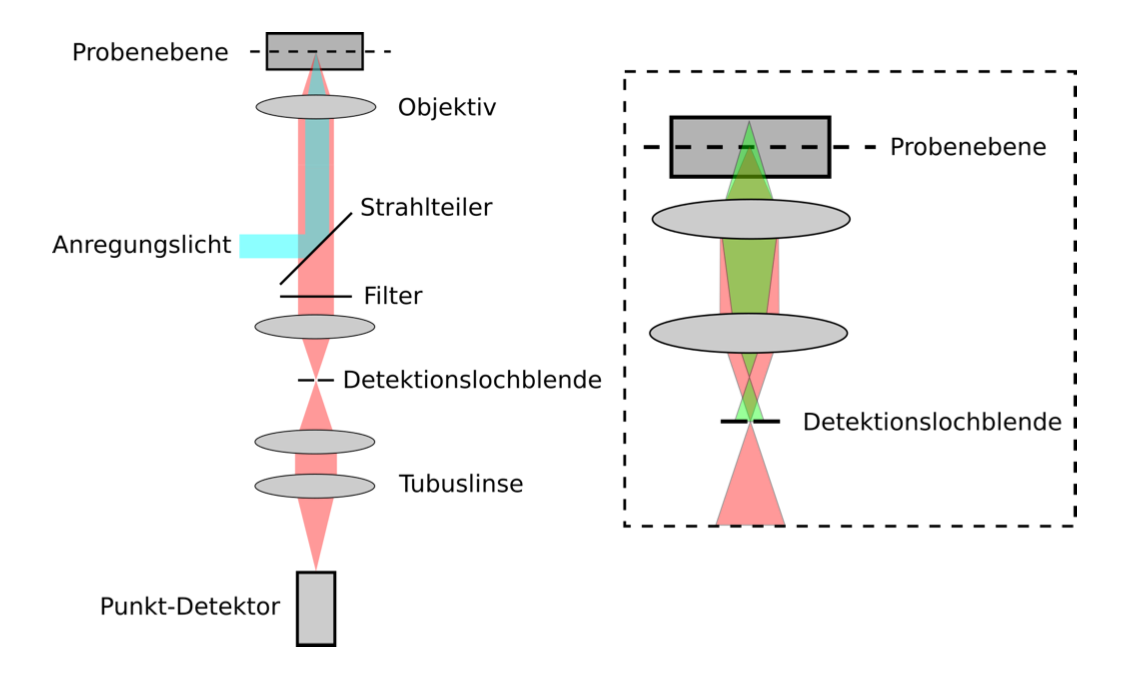
\includegraphics[scale=0.6]{Bilder/FzV/Konfokalmikroskop.png}
    \caption{Skizze des schematischen Aufbaus eines Konfokalmikroskop.\citep[vgl.][]{Anleitung} }
    \label{fig:Konfokalmikroskop}
   \end{figure}
Der Anregungsstrahl (in Abb. \ref{fig:Konfokalmikroskop} blau) trifft auf einen Strahlenteiler 
(z.B. ein halbdurchlässiger Spiegel), welcher diesen reflektiert und durch eine Linse gebündelt wird, 
sodass er im Brennpunkt auf die Probe trifft.\\
Der Detektionsstrahl (Abb. \ref{fig:Konfokalmikroskop} rot gekennzeichnet) wird durch 
die angeregte Probe ausgesendet. 
Der von der Probe ausgehende Strahl wird durch die oberste Linse parallelisiert und trifft
auf den Strahlenteiler, dieser lässt den Strahl transmittieren. Nach dem Strahlenteiler
ist, wie in der Skizze erkennbar, die Möglichkeit vorhanden einen Filter einzubauen. Dieser kann
die störenden Wellenlängen filtern und stoppen. 
Nach dem Filter befindet sich eine weitere Linse und die Detektionslochblende. Diese Blende sorgt
dafür, dass das Detektionsvolumen auf einen sehr kleinen Bereich eingeschränkt wird, d.h. die 
Strahlen aus dem hinteren Bereich der Probe gelangen nicht mehr zum Detektor. 
Nach der Blende trifft der Strahl auf die erste Tubuslinse, welche den Detektionsstrahl wieder parallelisiert, die 
zweite Tubuslinse fokussiert anschließend den Strahl auf den Punkt-Detektor, welcher
die einzelnen Photonen detektiert. \\
\subsection{Vor- bzw. Nachteile}
Der große Vorteil von Konfokalmikroskopie ist die Möglichkeit, 
unerwünschtes Hintergrundrauschen der Probe, meist Streulicht,
auf ein Minimum zu reduzieren, da durch eine Detektionslochblende nur 
Licht aus der konfokalen Ebene detektiert wird. 
Somit ist die axiale Auflösung im Vergleich zur konventionellen 
Mikroskopie viel besser.\\
Die Blende kann allerdings auch ein Nachteil sein, denn durch sie kann
es zu Beugungserscheinungen kommen, welche die Auflösung begrenzen.  
Als ein Nachteil könnte man zusätzlich noch anführen, dass durch die 
vielen Einzelaufnahmen die Probe eher langsam erfasst wird. 
\subsection{Alternative}
Wenn das Konfokalmikroskop zur Untersuchung der Probe nicht ausreichend ist, kann  
auch ein nicht konfokal Laser-Scanning-Microscope verwendet werden, diese benötigt die oben
genannte Blende nicht.
